\documentclass[letterpaper, 11pt]{article}
%\usepackage[hmargin = 1in, vmargin = 1in]{geometry}
\usepackage{amsmath}
\usepackage{amssymb}
\usepackage{enumitem}
\usepackage{mathrsfs}
\usepackage{tikz}
\usepackage{graphicx}
\usepackage{algorithmicx}
\usepackage{algpseudocode}
\usepackage{hyperref}
\hypersetup{
    colorlinks=true,
    linkcolor=blue,
    filecolor=magenta,      
    urlcolor=blue,
}
% \doublespacing
\setlength{\headheight}{14pt}
\usepackage{fancyhdr}
\pagestyle{fancy}
\rhead{Gabriel Wallace}
\lhead{Comp Sci 3130}

\newcommand{\card}{\text{Card}}
\newcommand{\N}{\mathbb{N}}
\newcommand{\R}{\mathbb{R}}
\newcommand{\Z}{\mathbb{Z}}
\newcommand{\Q}{\mathbb{Q}}

\newcommand{\inv}{^{-1}}
\newcommand{\abs}[1]{\lvert #1 \rvert}
\newcommand{\hwnumber}[1]{\medskip \noindent\textbf{#1.} \smallskip}
\newcommand{\hwnumbersec}[3]{\medskip \noindent\textbf{#1.} Section #2 \##3 \smallskip}
\newcommand{\Mod}[1]{\ \mathrm{mod}\ #1}
\newcommand{\Alg}[1]{\medskip \noindent\textbf{ALGORITHM} \( #1 \)} 
\newcommand{\To}{\textbf{ to }}

\begin{document}
\section{Theoretical Analysis}
The theoretical analysis of all the sorting algorithms were covered in class.
For reference, we have the table of the relevant sorting algorithms and their
efficiency for the best, worst, and average cases. 

\begin{center}
\begin{tabular}{l | l l l}
  Algorithm & Best  & Worst  & Average  \\
  \hline
  Selection & \(\Theta(n^2)\) & \(\Theta(n^2)\) & \(\Theta(n^2)\) \\
  Insertion & \(\Theta(n)\) & \(\Theta(n^2)\) & \(\Theta(n^2)\) \\
  Bubble & \(\Theta(n^2)\) & \(\Theta(n^2)\) & \(\Theta(n^2)\) \\
  Bubble (with swaps) & \(\Theta(1)\) & \(\Theta(n^2)\) & \(\Theta(n^2)\) \\
  Quick & \(\Theta(n \log n)\) & \(\Theta(n^2)\) & \(\Theta(n\log n)\) \\
  Merge & \(\Theta(n \log n)\) & \(\Theta(n\log n)\) & \(\Theta(n\log n)\) \\
\end{tabular}
\end{center}

\section{Empirical Analysis}
The following section covers the empirical analysis of the above sorting
algorithms. Due to memory issues (for more details see ), quicksort gets its
own section. All the algorithms were implemented in Python, and the source code
can be found on
\href{https://github.com/gwallace04/cs3130/blob/master/projects/proj2/proj2.py}
{GitHub}. The tables with the raw data for the analysis can be found in section
BLANK.

\subsection{Graphs and Discussion}
We have the graphs from all the algoritms below.
\begin{figure}[h]
  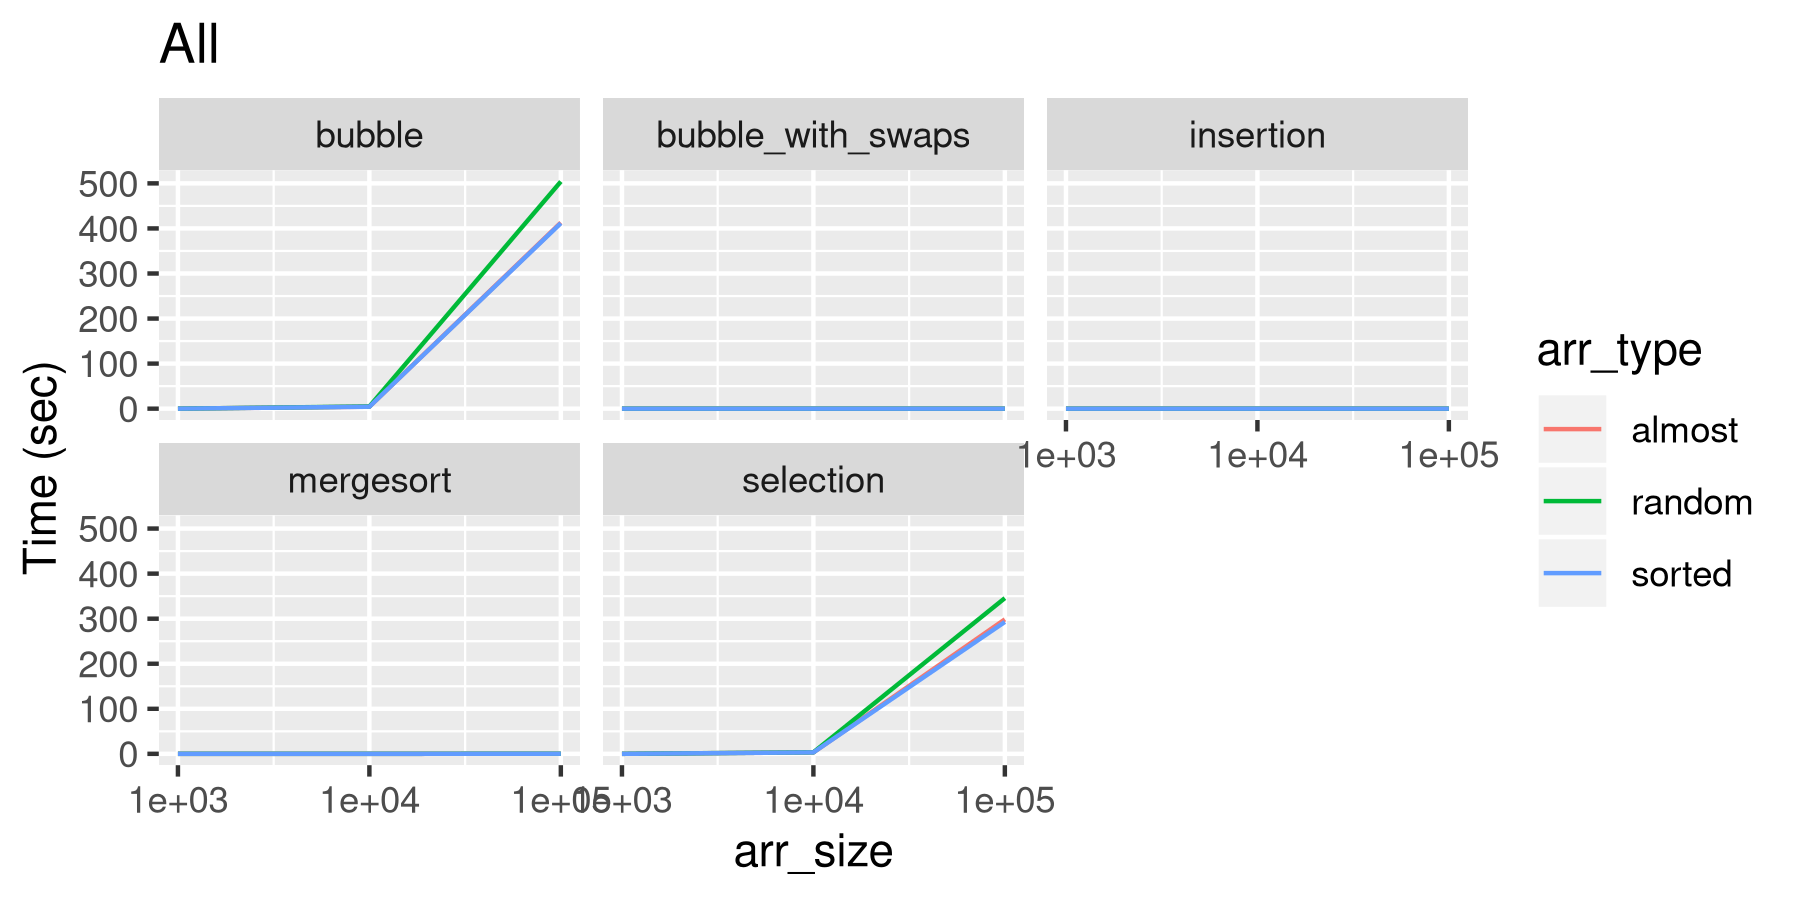
\includegraphics[width=\linewidth]{all.png}
\end{figure}

From the graphs we can see that bubble and selection sort grow much
quicker than the other sorting algoritms. So much so, that the scale of the
vertical axis makes it to where the other algorithms are basically a flat line.
To see the growth more clearly of the other sorting algoritms, we have separate
graphs. 

\begin{figure}[ht]
  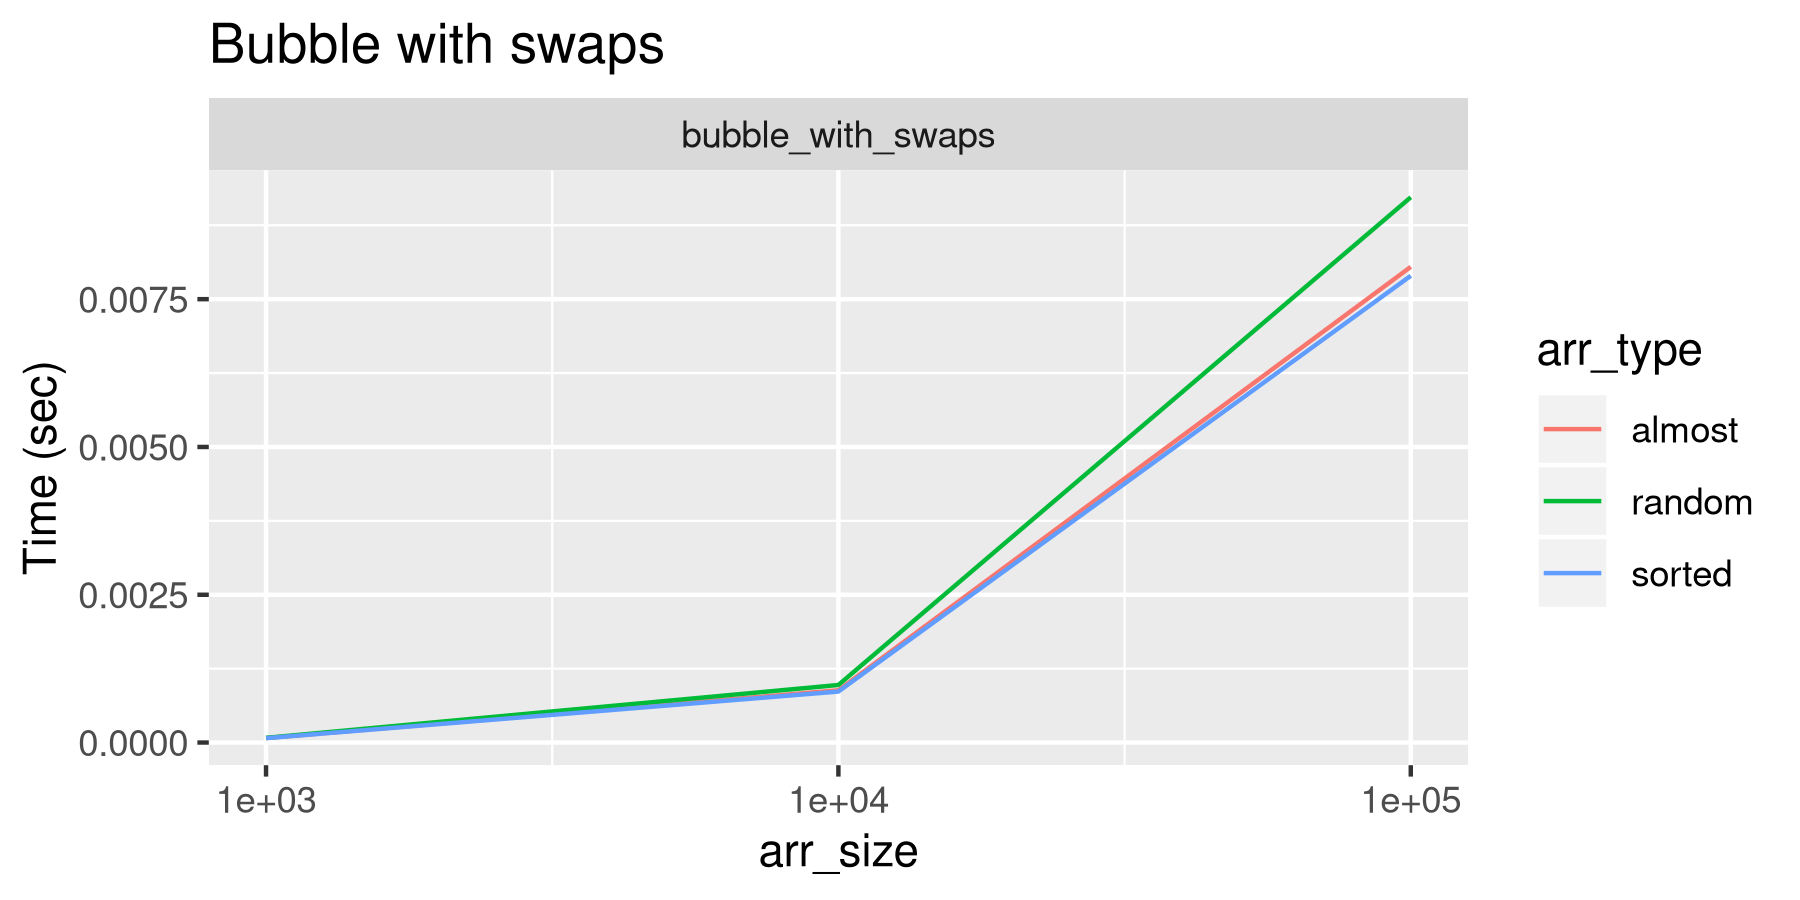
\includegraphics[width=\linewidth]{bubble_with_swaps.png}
\end{figure}

\begin{figure}[ht]
  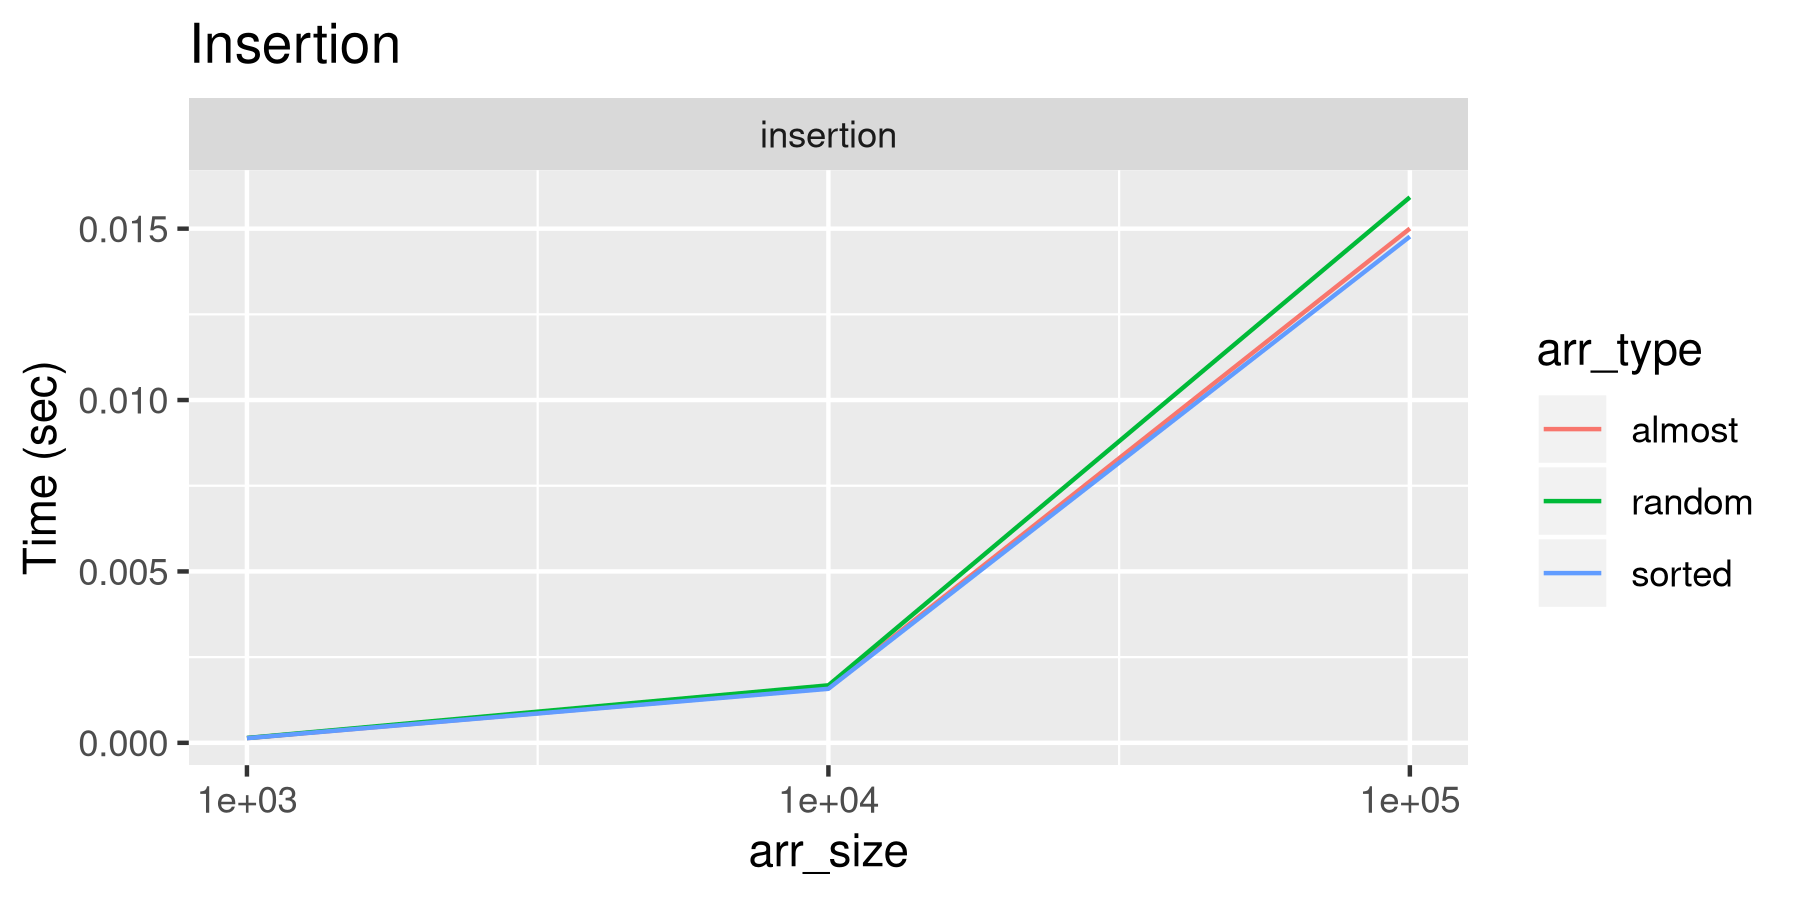
\includegraphics[width=\linewidth]{insertion.png}
\end{figure}

\begin{figure}[ht]
  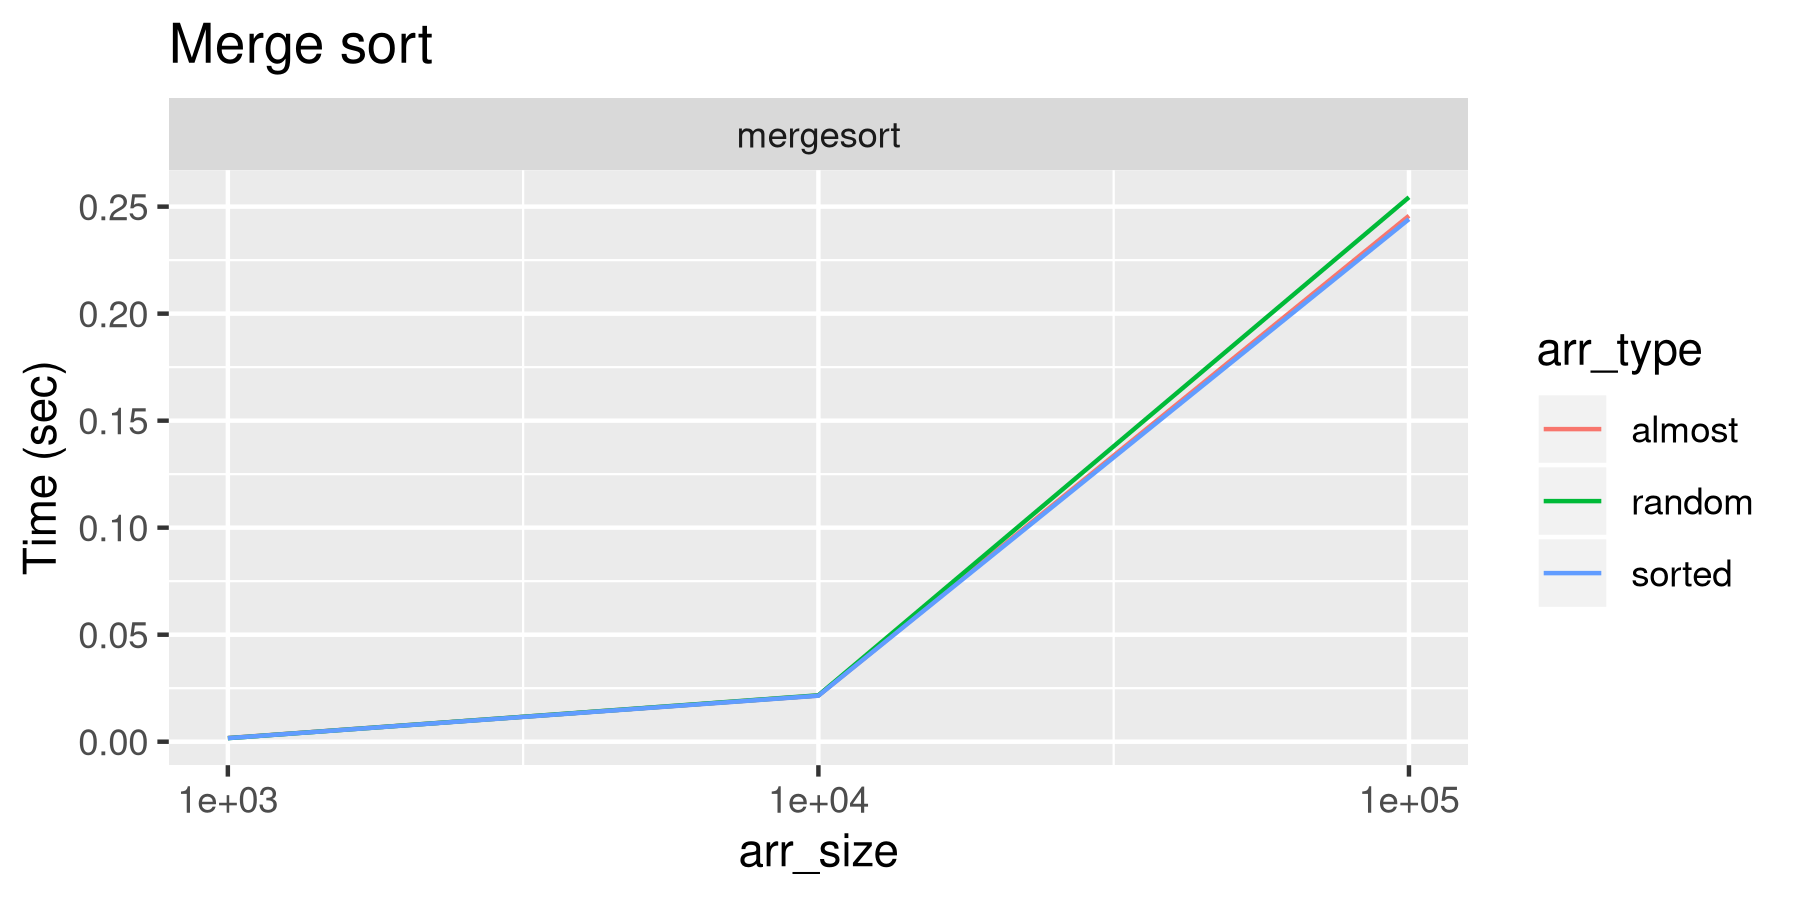
\includegraphics[width=\linewidth]{mergesort.png}
\end{figure}

It is hard to tell with only three data points, but we can see that all the
sorting algorithms have similar shapes, albeit with bubble and selection having
much steeper curves. 


\end{document}
